% LaTeX mintafájl szakdolgozat és diplomamunkáknak az
% SZTE Informatikai Tanszékcsoportja által megkövetelt
% formai követelményeinek megvalósításához
% Modosítva: 2011.04.28 Nemeth L. Zoltan
% A fájl használatához szükséges a magyar.ldf 2005/05/12 v1.5-ös vagy későbbi verziója
% ez letölthető a http://www.math.bme.hu/latex/ weblapról, a magyar nyelvű szedéshez
% Hasznos információk, linekek, LaTeX leírások a www.latex.lap.hu weboldalon vannak.
%

\documentclass[12pt]{report}

%Magyar nyelvi támogatás (Babel 3.7 vagy későbbi kell!)
\def\magyarOptions{defaults=hu-min}
\usepackage[magyar]{babel}

%Az ékezetes betűk használatához:
\usepackage{t1enc}% ékezetes szavak automatikus elválasztásához
\usepackage[utf8]{inputenc}% ékezetes szavak beviteléhez

% A formai kovetelmenyekben megkövetelt Times betűtípus használata:
\usepackage{times}

%Az AMS csomagjai
\usepackage{amsmath}
\usepackage{amssymb}
\usepackage{amsthm}

%A fejléc láblécek kialakításához:
\usepackage{fancyhdr}

%Természetesen további csomagok is használhatók,
%például ábrák beillesztéséhez a graphix és a psfrag,
%ha nincs rájuk szükség természetesen kihagyhatók.
\usepackage{graphicx}
\usepackage{psfrag}

\usepackage{setspace}

\usepackage{hyperref}
\hypersetup{
    colorlinks,
    citecolor=black,
    filecolor=black,
    linkcolor=black,
    urlcolor=black
}

%Tételszerű környezetek definiálhatók, ezek most fejezetenként együtt számozódnak, pl.
\newtheorem{tét}{Tétel}[chapter]
\newtheorem{defi}[tét]{Definíció}
\newtheorem{lemma}[tét]{Lemma}
\newtheorem{áll}[tét]{Állítás}
\newtheorem{köv}[tét]{Következmény}

%Ha a megjegyzések és a példak szövegét nem akarjuk dőlten szedni, akkor
%az alábbi parancs után kell őket definiální:
\theoremstyle{definition}
\newtheorem{megj}[tét]{Megjegyzés}
\newtheorem{pld}[tét]{Példa}

%Margók:
\hoffset -1in
\voffset -1in
\oddsidemargin 35mm
\textwidth 150mm
\topmargin 15mm
\headheight 10mm
\headsep 5mm
\textheight 237mm

\begin{document}


%%%%%%%%%%%%%%%%%%%%%%%%%%%%%%%%%%%%%%%%%%%%%%%%%%%%%%%%%%%%%%%%%%%%%%
%%   Címlap                                                         %%
%%%%%%%%%%%%%%%%%%%%%%%%%%%%%%%%%%%%%%%%%%%%%%%%%%%%%%%%%%%%%%%%%%%%%%

    %A FEJEZETEK KEZDŐOLDALAINAK FEJ ÉS LÁBLÉCE:
    %a plain oldalstílust kell átdefiniálni, hogy ott ne legyen fejléc:
    \fancypagestyle{plain}{%
    %ez mindent töröl:
    \fancyhf{}
    % a láblécbe jobboldalra kerüljön az oldalszám:
    \fancyfoot[R]{\thepage}
    %elválasztó vonal sem kell:
    \renewcommand{\headrulewidth}{0pt}
    }

    %A TÖBBI OLDAL FEJ ÉS LÁBLÉCE:
    \pagestyle{fancy}
    \fancyhf{}
    \fancyhead[L]{A diplomamunka címe}
    \fancyfoot[R]{\thepage}


    %A címoldalra se fej- se lábléc nem kell:
    \thispagestyle{empty}

    \begin{center}
    \vspace*{1cm}
    {\Large\bf Szegedi Tudományegyetem}

    \vspace{0.5cm}

    {\Large\bf Informatikai Tanszékcsoport}

    \vspace*{3.8cm}


    {\LARGE\bf A diplomamunka címe}


    \vspace*{3.6cm}

    {\Large Diplomamunka}
    % vagy {\Large Szakdolgozat}

    \vspace*{4cm}

    %Értelemszerűen megváltoztatandó:
    {\large
    \begin{tabular}{c@{\hspace{4cm}}c}
    \emph{Készítette:}     &\emph{Témavezető:}\\
    \bf{Ledán Szilárd}  &\bf{Dr. Kiss Ákos}\\
    informatika szakos     & adjunktus\\
    hallgató &
    \end{tabular}
    }

    \vspace*{2.3cm}

    {\Large
    Szeged
    \\
    \vspace{2mm}
    2016
    }
    \end{center}


    % 1.5-ös sorköz:
    % ezt javasolják:  \linespread{1.25}
    % és ez bevált, de ehhez kellett a \usepackage{setspace} csomag betöltése.
    \onehalfspacing


%%%%%%%%%%%%%%%%%%%%%%%%%%%%%%%%%%%%%%%%%%%%%%%%%%%%%%%%%%%%%%%%%%%%%%
%%   Tartalomjegyzék                                                %%
%%%%%%%%%%%%%%%%%%%%%%%%%%%%%%%%%%%%%%%%%%%%%%%%%%%%%%%%%%%%%%%%%%%%%%

    \tableofcontents


%%%%%%%%%%%%%%%%%%%%%%%%%%%%%%%%%%%%%%%%%%%%%%%%%%%%%%%%%%%%%%%%%%%%%%
%%   Feladatkiírás                                                  %%
%%%%%%%%%%%%%%%%%%%%%%%%%%%%%%%%%%%%%%%%%%%%%%%%%%%%%%%%%%%%%%%%%%%%%%


    %A \chapter* parancs nem ad a fejezetnek sorszámot
    \chapter*{Feladatkiírás}
    %A tartalomjegyzékben mégis szerepeltetni kell, mint szakasz(section) szerepeljen:
    \addcontentsline{toc}{section}{Feladatkiírás}

A témavezető által megfogalmazott feladatkiírás. Önálló oldalon szerepel.


%%%%%%%%%%%%%%%%%%%%%%%%%%%%%%%%%%%%%%%%%%%%%%%%%%%%%%%%%%%%%%%%%%%%%%
%%   Tartalmi összefoglaló                                          %%
%%%%%%%%%%%%%%%%%%%%%%%%%%%%%%%%%%%%%%%%%%%%%%%%%%%%%%%%%%%%%%%%%%%%%%

    \chapter*{Tartalmi összefoglaló}
    \addcontentsline{toc}{section}{Tartalmi összefoglaló}

A tartalmi összefoglalónak tartalmaznia kell (rövid, legfeljebb egy oldalas, összefüggő megfogalmazásban)
a következőket: a téma megnevezése, a megadott feladat megfogalmazása - a feladatkiíráshoz viszonyítva-,
a megoldási mód, az alkalmazott eszközök, módszerek, az elért eredmények, kulcsszavak (4-6 darab).

Az összefoglaló nyelvének meg kell egyeznie a dolgozat nyelvével. Ha a dolgozat idegen nyelven készül,
magyar nyelvű tartalmi összefoglaló készítése is kötelező (külön lapon), melynek terjedelmét a TVSZ szabályozza.

    \subsubsection*{A téma megnevezése}

A \textit{W3C} (World Wide Web Consortium) által \textit{Canvas 2D
Context} néven 2015-ben elfogadott ajánlás\footnote{} Path részének
megvalósítása \textit{OpenGL-ES 2.0} alapokon.

    \subsubsection*{A megadott feladat megfogalmazása}

    \subsubsection*{A megoldásmód}

    \subsubsection*{Alkalmazott eszközök, módszerek}

    \subsubsection*{Elért eredmények}

    \subsubsection*{Kulcsszavak}

grafika, path, canvas-2D-context, OpenGL-ES 2.0


%%%%%%%%%%%%%%%%%%%%%%%%%%%%%%%%%%%%%%%%%%%%%%%%%%%%%%%%%%%%%%%%%%%%%%
%%   Bevezetés                                                      %%
%%%%%%%%%%%%%%%%%%%%%%%%%%%%%%%%%%%%%%%%%%%%%%%%%%%%%%%%%%%%%%%%%%%%%%

    \chapter*{Bevezetés}
    \addcontentsline{toc}{section}{Bevezetés}

Egyre nagyobb a jelentősége az erős, gyors és energiahatékony grafikus
renderelő motoroknak.


%%%%%%%%%%%%%%%%%%%%%%%%%%%%%%%%%%%%%%%%%%%%%%%%%%%%%%%%%%%%%%%%%%%%%%
%%   Háttér                                                         %%
%%%%%%%%%%%%%%%%%%%%%%%%%%%%%%%%%%%%%%%%%%%%%%%%%%%%%%%%%%%%%%%%%%%%%%

    \chapter{Háttér}
    \addcontentsline{toc}{section}{Háttér}


%%%%%%%%%%%%%%%%%%%%%%%%%%%%%%%%%%%%%%%%%%%%%%%%%%%%%%%%%%%%%%%%%%%%%%
%%   Path API                                                       %%
%%%%%%%%%%%%%%%%%%%%%%%%%%%%%%%%%%%%%%%%%%%%%%%%%%%%%%%%%%%%%%%%%%%%%%

    \chapter{Path belső API}

    \begin{figure}[h]
    \centering
    \psfrag{t}[c][c]{$q_0$}
    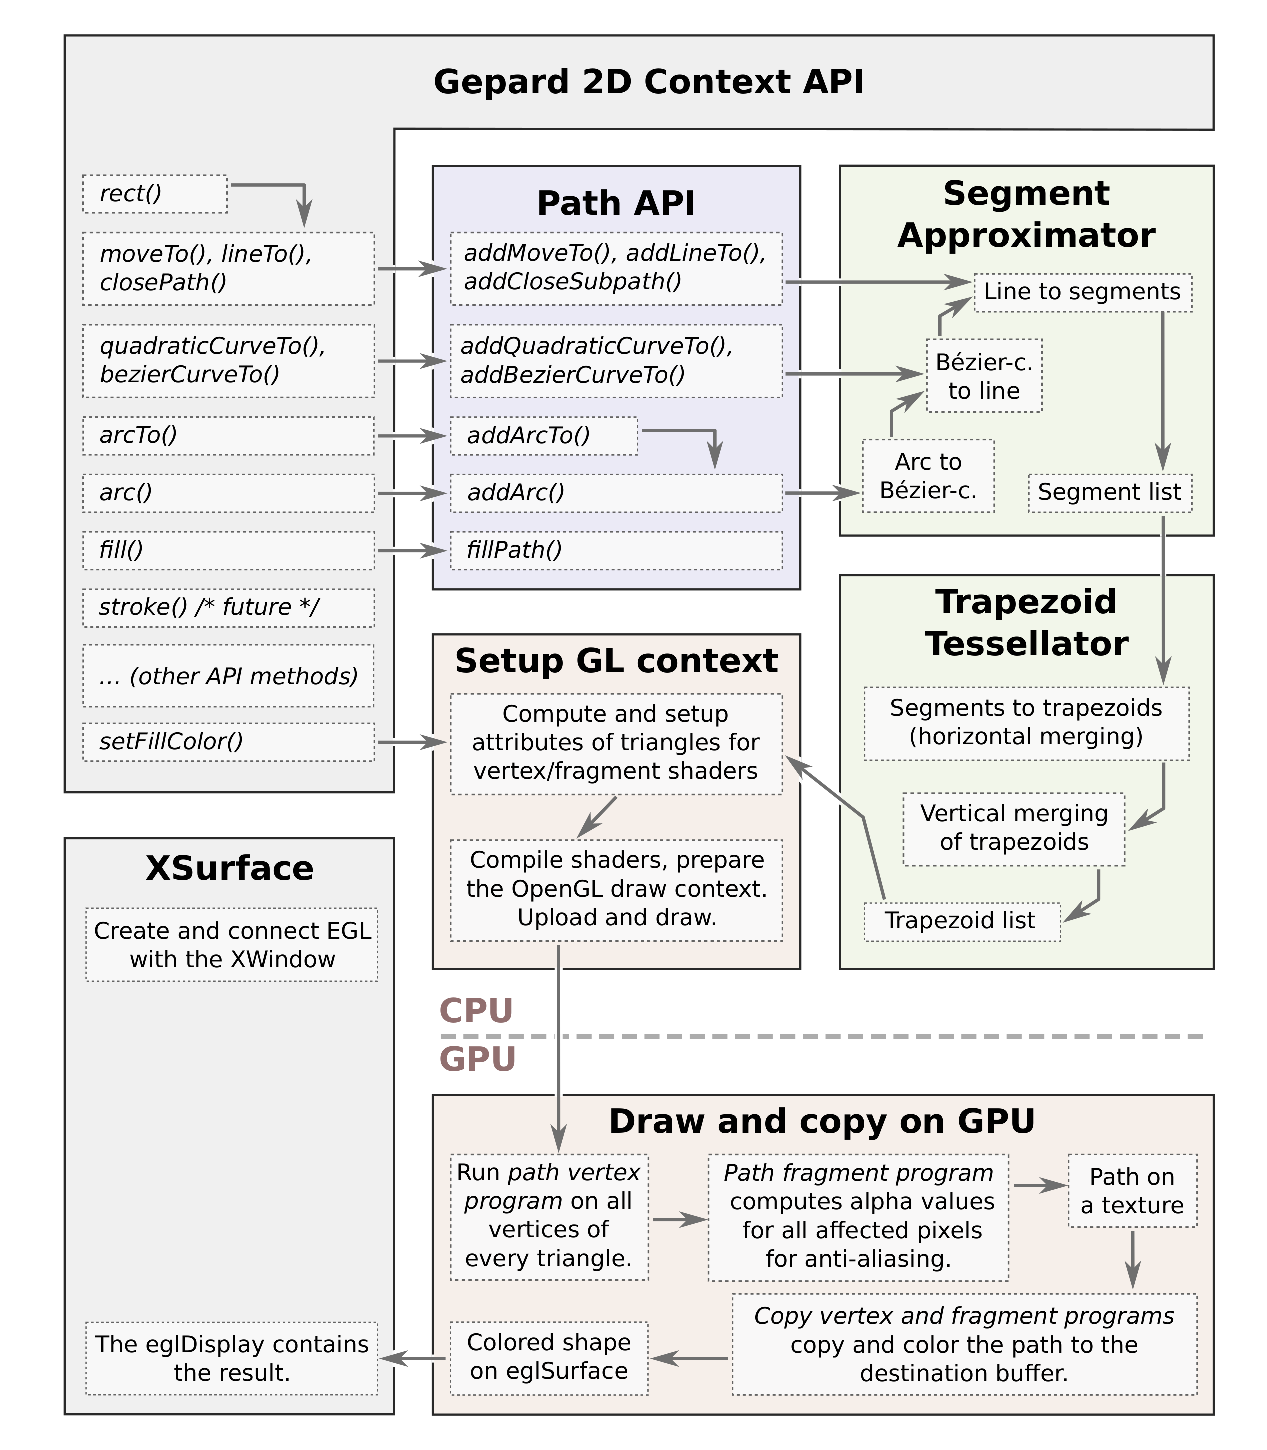
\includegraphics[scale=0.7]{dataflow.eps}
    \caption{\label{dataflow-diagram} A rajzolás folyamata}
    \end{figure}


%%%%%%%%%%%%%%%%%%%%%%%%%%%%%%%%%%%%%%%%%%%%%%%%%%%%%%%%%%%%%%%%%%%%%%
%%   Konklúzió                                                      %%
%%%%%%%%%%%%%%%%%%%%%%%%%%%%%%%%%%%%%%%%%%%%%%%%%%%%%%%%%%%%%%%%%%%%%%

    \chapter{Konklúzió}
    \addcontentsline{toc}{section}{Konklúzió}


%%%%%%%%%%%%%%%%%%%%%%%%%%%%%%%%%%%%%%%%%%%%%%%%%%%%%%%%%%%%%%%%%%%%%%
%%   Irodalomjegyzék                                                %%
%%%%%%%%%%%%%%%%%%%%%%%%%%%%%%%%%%%%%%%%%%%%%%%%%%%%%%%%%%%%%%%%%%%%%%

    \begin{thebibliography}{9}

    \end{thebibliography}


%%%%%%%%%%%%%%%%%%%%%%%%%%%%%%%%%%%%%%%%%%%%%%%%%%%%%%%%%%%%%%%%%%%%%%
%%   Nyilatkozat                                                    %%
%%%%%%%%%%%%%%%%%%%%%%%%%%%%%%%%%%%%%%%%%%%%%%%%%%%%%%%%%%%%%%%%%%%%%%

    \chapter*{Nyilatkozat}
    %Egy üres sort adunk a tartalomjegyzékhez:
    \addtocontents{toc}{\ }
    \addcontentsline{toc}{section}{Nyilatkozat}
    %\hspace{\parindent}

    % A nyilatkozat szövege más titkos és nem titkos dolgozatok esetében.
    % Csak az egyik típusú nyilatkozatnak kell a dolgozatban szerepelni
    % A pontok helyére az adatok értelemszerűen behelyettesítendők és
    % a szakdolgozat /diplomamunka szó megfelelően kiválasztandó.


    % A nyilatkozat szövege TITKOSNAK NEM MINŐSÍTETT dolgozatban a következő:
    % A pontokkal jelölt szövegrészek értelemszerűen a szövegszerkesztőben és
    % nem kézzel helyettesítendők:

    \noindent

Alulírott \makebox[4cm]{\dotfill} szakos hallgató, kijelentem, hogy a dolgozatomat a Szegedi Tudományegyetem, Informatikai Tanszékcsoport \makebox[4cm]{\dotfill} Tanszékén készítettem, \makebox[4cm]{\dotfill} diploma megszerzése érdekében.

Kijelentem, hogy a dolgozatot más szakon korábban nem védtem meg, saját munkám eredménye, és csak a hivatkozott forrásokat (szakirodalom, eszközök, stb.) használtam fel.

Tudomásul veszem, hogy szakdolgozatomat / diplomamunkámat a Szegedi Tudományegyetem Informatikai Tanszékcsoport könyvtárában, a helyben olvasható könyvek között helyezik el.

    \vspace*{2cm}

    \begin{tabular}{lc}
    Szeged, \today\
    \hspace{2cm} & \makebox[6cm]{\dotfill} \\
    & aláírás \\
    \end{tabular}


%%%%%%%%%%%%%%%%%%%%%%%%%%%%%%%%%%%%%%%%%%%%%%%%%%%%%%%%%%%%%%%%%%%%%%
%%   Köszönetnyilvánítás                                            %%
%%%%%%%%%%%%%%%%%%%%%%%%%%%%%%%%%%%%%%%%%%%%%%%%%%%%%%%%%%%%%%%%%%%%%%

    \chapter*{Köszönetnyilvánítás}
    \addcontentsline{toc}{section}{Köszönetnyilvánítás}

Ezúton szeretnék köszönetet mondani \textbf{X. Y-nak} ezért és ezért \ldots


\end{document}
